\documentclass{article}
\usepackage[utf8]{inputenc}
\usepackage[spanish]{babel}
\usepackage{listings}
\usepackage{graphicx}
\graphicspath{ {images/} }
\usepackage{cite}

\begin{document}

\begin{titlepage}
    \begin{center}
        \vspace*{1cm}
            
        \Huge
        \textbf{Seguimiento de instrucciones}
            
        \vspace{0.5cm}
        \LARGE
        desafió de la pirámide 
            
        \vspace{1.5cm}
            
        \textbf{Rolman David Echavarria Prince}
            
        \vfill
            
        \vspace{0.8cm}
            
        \Large
        Departamento de Ingeniería Electrónica y Telecomunicaciones\\
        Universidad de Antioquia\\
        Medellín\\
        Marzo de 2021
            
    \end{center}
\end{titlepage}

\tableofcontents
\newpage
\section{Introducción}\label{intro}
Demostrar la capacidad motriz de un ejercicio con una sola mano; buscando formar con dos cartas una pirámide sobre una hoja, el objetivo de ver como el participante logra comprender las instrucciones.

\section{Sección de contenido} \label{contenido}
Desafió de formar una pirámide con dos cartas sobre una hoja.
\subsection{materiales}
\begin{enumerate}
    \item Dos cartas (Preferiblemente iguales).
    \item Una hoja en condiciones normales.
    \item Disponer de una superficie horizontal plana (Preferiblemente una mesa).
\end{enumerate}
\subsection{Sugerencias}
\begin{enumerate}
    \item [-]El ángulo superior que une las dos cartas formen aproximadamente 40º.
    \item[-]Los lados cortos superiores que unen las dos cartas alineadas, quede uno sobre el otro justamente, considerar esto si una carta es más densa que la otra.
\end{enumerate}
\subsection{procedimiento}
El desafío busca saber si el participante comprende las indicaciones hacia el objetivo y lograr una destreza realizando este ejercicio.
\begin{enumerate}
    \item [-]Sobre una parte despejada de la mesa tendremos inicialmente la hoja con las dos cartas, que estarán las cartas debajo de la hoja.
     \item [-]Escoger una mano (para este ejemplo la derecha).
     \item [-]Con la mano levantar la hoja sin comprometer su estado, dejarla sobre la misma mesa sin volver a tapar las cartas.
     \item [-]Tomar ambas cartas y dejarlas sobre el área central de la hoja.
     \item [-]Deslizar suavemente la hoja sobre la mesa para llevarla cerca a usted en una posición cómoda para realizar el desafío.  
     \item [-]Como las cartas en general son rectangulares con sus respectivos lados cortos y largos, tomar las cartas que queden juntas y alineadas.
     \item [-]Con la yema de los dedos sujetaremos las cartas, no es necesario involucrar al meñique.
     \item [-]Dedo índice sobre lado corto superior, pulgar en lado largo izquierdo, anular y medio en el lado largo derecho y lado corto inferior sobre la hoja.
     \item [-]Tendrás una carta que mira tu palma y otra exterior, las cartas deben estar de forma normal respecto a la hoja.
     \item [-]Aplicamos una presión con el índice, justamente para que no se corra en la separación.
     \item [-]Buscamos separarlas con ayuda de pulgar, anular y medio desde la parte inferior solamente, la parte superior seguirá unida y será la cima de la pirámide.
     \item [-]Recordar las sugerencias.
     \item [-]Cuando consideremos una estabilidad en la estructura, soltarlas suavemente, logrando el objetivo dado.

\end{enumerate}
\subsection{Citación}
Portal de donde se extrajo el material como plantilla \cite{classroom}.



\section{Ayuda ilustrativa} \label{imagenes}

En la Figura (\ref{fig:objetivofinal}), se ilustra el objetivo deseado del desafió.

\begin{figure}[h]
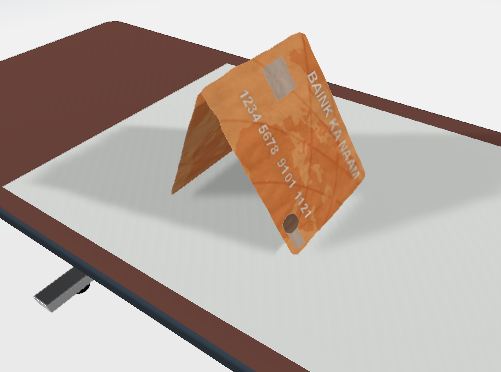
\includegraphics[width=4cm]{objetivofinal.png}
\centering
\caption{desafió de la pirámide}
\label{fig:objetivofinal}
\end{figure}


\bibliographystyle{IEEEtran}
\bibliography{references}

\end{document}
